
%
%
%

\begin{frame}[t,allowframebreaks]{CNN Layer Types: Convolution -}

    In a \index{CNN}\index{convolutional neural network}\gls{cnn},
    parameters are organised in a number of 
    \index{filter}\glspl{filter} (or \index{kernel}\glspl{kernel}).
    \begin{itemize}
        \item
        These parameters are the \gls{cnn} equivalent of weights and biases.
        \item
        The number of \glspl{filter} controls the {\bf capacity of the model}.
        \item 
        The \glspl{filter} are {\bf learnt during training}.
        \item 
        A \gls{filter} is a {\bf feature detector}.
    \end{itemize}

    \vspace{0.2cm}

    A \gls{filter} applied to a layer generates 
    a \index{feature map}\gls{feature map} of the next layer.
    \begin{itemize}
        \item
        The \glspl{filter} have the {\bf same grid structure} as the layer they are applied to,
        but they are {\bf much smaller in size} (and usually square).
        \item
        The number of filters in a layer determines the depth of the next layer.
    \end{itemize}

    \begin{blockexample}{}
        \small
        The {\bf depth of a layer} should \underline{not be confused} 
        with the {\bf depth of the network}.
        \begin{itemize}
          \item The depth of a layer is the number of feature maps in that layer.
          \item The depth of the network is the number of layers in the network.
        \end{itemize}
    \end{blockexample}

    \framebreak

    A {\bf single feature} is generated by 
    \begin{itemize}
      \item 
      overlaying a \gls{filter} at a specific position on a layer, and
      \item 
      convolving the filter with the subset of the layer spanned by the filter.
    \end{itemize}

    \begin{columns}
        \begin{column}{0.60\textwidth}
            \begin{center}
                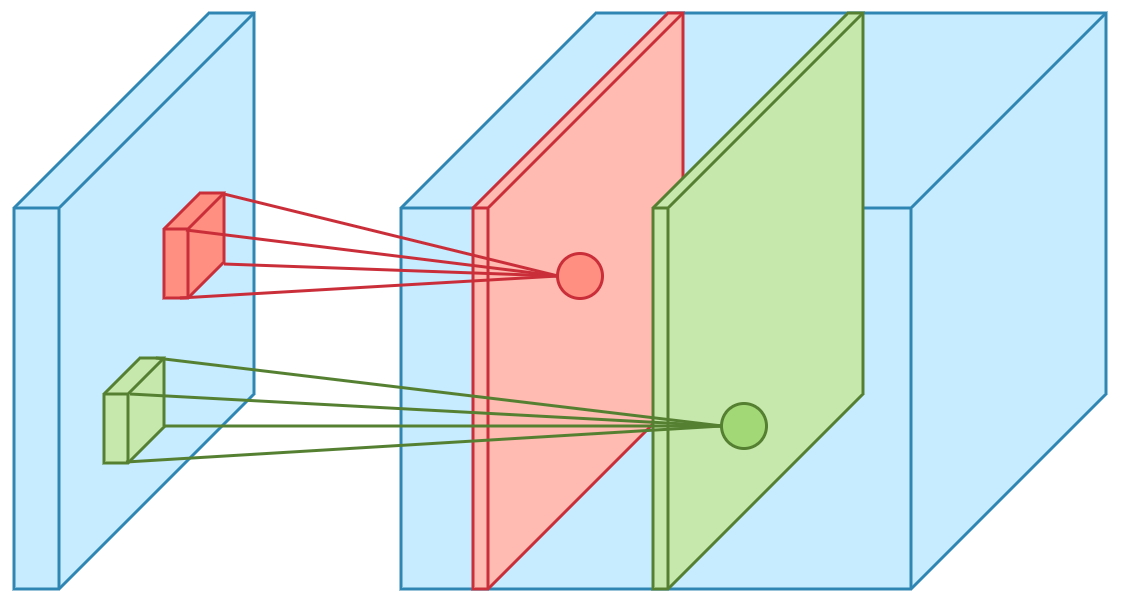
\includegraphics[width=0.97\textwidth]
                  {./images/cnn/convolution/dertat17_convolution_illustration.png}\\
                {\scriptsize 
                  \color{col:attribution} 
                  Image from \cite{TowardsDataScience:AppliedDL4}}\\    
            \end{center}      
        \end{column}
        \begin{column}{0.40\textwidth}
            {\bf Sliding a single filter} over all possible positions generates
            a complete \index{feature map}\gls{feature map} of the input layer.\\
            \vspace{0.2cm}
            The number of \glspl{feature map} (i.e. the depth of the layer
            produced by the convolution operations)
            is {\bf determined by the number of filters}.\\
        \end{column}
    \end{columns}
    \vspace{0.2cm}
    The output \glspl{feature map} can be further processed in subsequent layers,
    some of which can be convolutional.

    \framebreak

    \begin{columns}[t]
        \begin{column}{0.50\textwidth}
            \vspace{-0.4cm}
            \begin{center}
                {\scriptsize A simple concrete example is shown below.}\\
                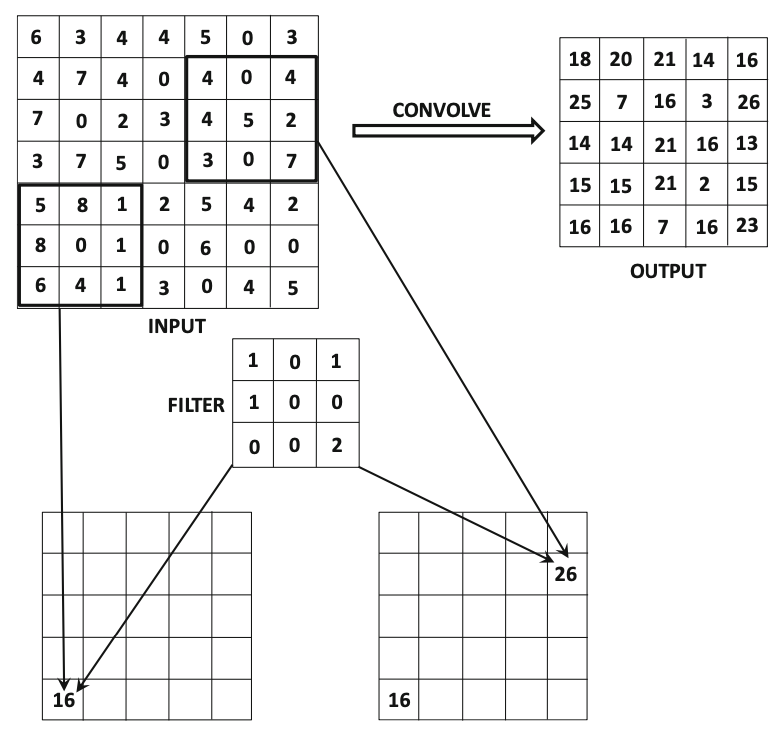
\includegraphics[width=1.00\textwidth]
                  {./images/cnn/convolution/aggarwal_convolution_illustration_1.png}\\
                {\scriptsize 
                  \color{col:attribution} 
                  Image reproduced from \cite{Aggarwal:2018SpringerDL} (Fig 8.2)}\\    
            \end{center}      
        \end{column}
        \begin{column}{0.50\textwidth}
        {\scriptsize
            Assume that we have:
            \begin{itemize}
            {\scriptsize        
              \item 
              a greyscale input image represented by a 7x7 array
              (depth is 1 as there is a single colour channel), 
              and 
              \item
              a single filter represented by a 3x3 array
            }
            \end{itemize}
            as shown on the left.\\
            \vspace{0.1cm}
            The feature map (output) shown 
            is computed by sliding the filter over the image and, at each position,
            performing a convolution operation.\\
            \vspace{0.1cm}
            If we place the filter on the bottom-left corner of the 
            image, as shown, the convolution of the 3x3 filter 
            with the corresponding 3x3 subset of the image, yields:
            \vspace{-0.2cm}
            \begin{center} 
            (5,8,1,8,0,1,6,4,1)$\cdot$(1,0,1,1,0,0,0,0,2) =\\ 
            5+1+8+2 = 16\\
            \end{center} 
            \vspace{-0.2cm}
            There are 5 different positions in each direction
            where the 3x3 filter fits inside the 7x7 image.
            Therefore, the feature map has a reduced size (5x5) with respect
            to the input image.\\
        }
        \end{column}
    \end{columns}

    \framebreak

    %\vspace{-1.0cm}
    Convolutions {\bf increase the receptive field} of their output feature maps.
    Deeper layers, capture characteristics over larger spatial regions.
    \begin{center}
        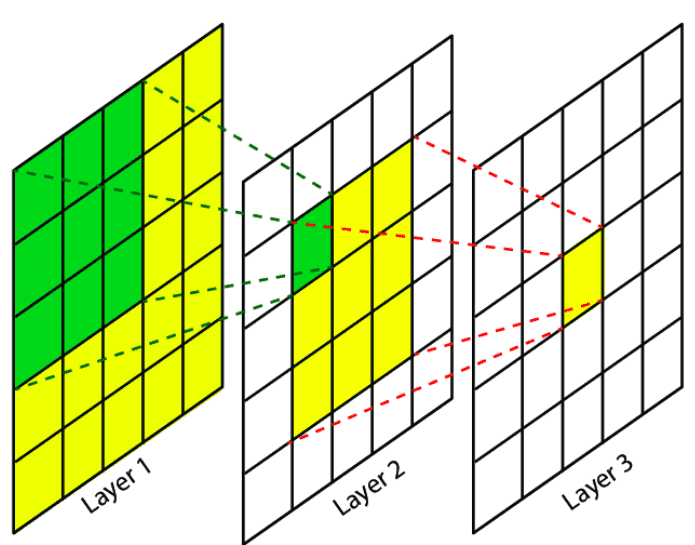
\includegraphics[width=0.57\textwidth]
          {./images/cnn/receptive_field/lin17_3_layers_receptive_field.png}\\
        {\scriptsize 
          Increased receptive field of deeper layers. 
          \color{col:attribution} 
          Image reproduced from \cite{Lin:2017rf}}\\    
    \end{center}      

    \framebreak

    %\vspace{-0.4cm}
    Convolution operations: 
    \begin{itemize}
        \item 
        {\bf reduce the spatial size of the output layer}, and,
        \item 
        typically, they {\bf increase its depth} 
        since an increasing number of filters is required 
        in deeper layers to capture more complex patterns.\\
    \end{itemize}

    \begin{center}
        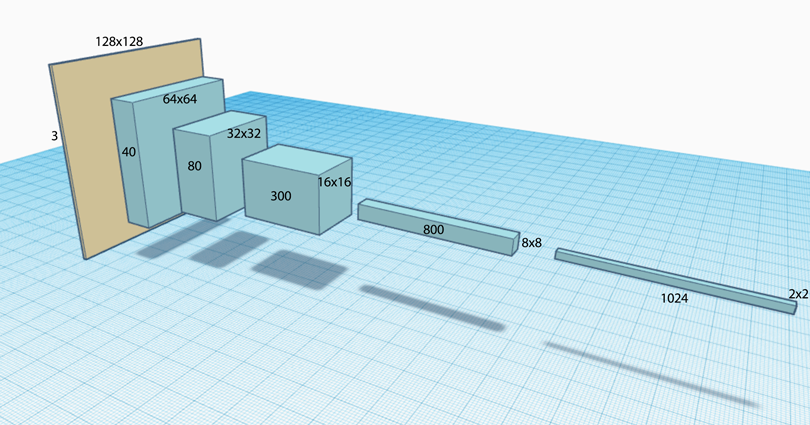
\includegraphics[width=0.72\textwidth]
            {./images/cnn/convolution/hui17_convolutional_pyramid_1.png}\\
        {\scriptsize
            The convolutional pyramid. 
            \color{col:attribution} 
            Image reproduced from \cite{HuiBlog:CNNTutorial}}\\    
    \end{center}

    \framebreak

    The {\bf reduction of spatial size of 
    \index{feature map}\glspl{feature map} is undesirable.}\\
    \vspace{0.2cm}
    
    {\bf It loses information} from pixels near or at the boundary 
    of the input layer, as their contribution is not well represented in the next layer.
    \begin{itemize}
        \item The problem is exacerbated over successive convolutional layers.\\
    \end{itemize}
    \vspace{0.2cm}

    The issue is addressed using \index{padding}{\bf \gls{padding}}, 
    i.e. {\bf adding new pixels around the borders} of a \gls{feature map}.\\
    \begin{itemize}
        \item
        \Gls{padding} allows the \index{filter}\glspl{filter} used by a convolutional layer
        to (partially) stick out from the borders of the actual input \gls{feature map}.\\
        \item
        The added pixels {\bf do not contribute in convolution} operations.\\
    \end{itemize}
    \vspace{0.2cm}

    There are {\bf different types of padding}.\\

    \framebreak

    There are different types of \index{padding}\gls{padding}:
    \begin{itemize}
        \item 
        \index{valid padding}\Gls{valid padding}: This is the same as not using padding.
        \item 
        \index{half padding}\Gls{half padding}:
        \item 
        \index{full padding}\Gls{full padding}:
    \end{itemize}


    \framebreak

    Strides

    \framebreak

    Activation

    \framebreak

    Examples
    
\end{frame}